\documentclass{beamer}

\usepackage{tikz}

\usepackage{listings}
% \newcommand{\titleimage}{KeYBeamer2}

\usetheme{kit}
\beamertemplatenavigationsymbolsempty

\newcommand{\KeY}{Ke\kern-.1em Y}
\newcommand{\kit}[1]{\textcolor{kit-green100}{#1}}
\newcommand{\kitblue}[1]{\textcolor{kit-blue100}{#1}}

\title{The \KeY-verified Verified Keyserver}

\lstset{ 
  backgroundcolor=\color{white},   % choose the background color; you must add \usepackage{color} or \usepackage{xcolor}; should come as last argument
  basicstyle=\tiny\ttfamily,               % the size of the fonts that are used for the code
  breakatwhitespace=false,         % sets if automatic breaks should only happen at whitespace
  breaklines=true,                 % sets automatic line breaking
  captionpos=b,                    % sets the caption-position to bottom
  commentstyle=\color{mygreen},    % comment style
  deletekeywords={...},            % if you want to delete keywords from the given language
  escapeinside={\%*}{*)},          % if you want to add LaTeX within your code
  extendedchars=true,              % lets you use non-ASCII characters; for 8-bits encodings only, does not work with UTF-8
  %firstnumber=1000,                % start line enumeration with line 1000
  frame=single,	                   % adds a frame around the code
  keepspaces=true,                 % keeps spaces in text, useful for keeping indentation of code (possibly needs columns=flexible)
  keywordstyle=\color{blue},       % keyword style
  language=Java,                 % the language of the code
  morekeywords={*,invariant,\\forall,requires,ensures,normal_behaviour},            % if you want to add more keywords to the set
  %numbers=left,                    % where to put the line-numbers; possible values are (none, left, right)
  numbersep=5pt,                   % how far the line-numbers are from the code
  %numberstyle=\tiny\color{mygray}, % the style that is used for the line-numbers
  rulecolor=\color{black},         % if not set, the frame-color may be changed on line-breaks within not-black text (e.g. comments (green here))
  %showspaces=false,                % show spaces everywhere adding particular underscores; it overrides 'showstringspaces'
  %showstringspaces=false,          % underline spaces within strings only
  %showtabs=false,                  % show tabs within strings adding particular underscores
  %stepnumber=2,                    % the step between two line-numbers. If it's 1, each line will be numbered
  %stringstyle=\color{mymauve},     % string literal style
  %tabsize=2,	                   % sets default tabsize to 2 spaces
  %title=\lstname                   % show the filename of files included with \lstinputlisting; also try caption instead of title
}




\date{27 April 2020}
\author[de Gouw, Ulbrich, Weigl]{Stijn de Gouw (Open University, NL),
  Mattias Ulbrich, Alexander Weigl}

\institute{Institute for Theoretical Informatics}

\begin{document}

\selectlanguage{english}

\begin{frame}
\titlepage
\end{frame}

\begin{frame}{Our program verifier \KeY}
  \vspace{-1.5cm}
  \begin{center}
    \begin{tikzpicture}
      \node at (0,0) { 
\includegraphics[height=8cm]{key} };
      \node at (-2.5,2.5) {\large Deductive verification};
      \node[text width=3cm] at (-4.5,.5) {\large Java Modeling\\Language (JML)};
      \node[text width=3cm] at (4,-1.5) {\large Modular\\Reasoning};
      \node at (-3.5,-1.5) {\large User Interaction Concepts};
      \node at (2,2.5) {\large 100\% Java Card};
      \node at (-2,-2.5) {\large Test case generation};
      \node at (2,-3) {\large Secure Information Flow};
      \node at (0,-4) {\footnotesize collaboration with
        TU Darmstadt and Chalmers University, Gothenburg};
    \end{tikzpicture}
  \end{center}\vspace{-1ex}
\end{frame}

\begin{frame}
  \frametitle{Modelling HAGRID in \KeY}

  We present two formalisations of the HAGRID framework as spec'ed and
  verif'ed Java implementations:
  \pause
  
  \begin{block}{The \textbf{automatic} model}
%  \footnotesize
    \begin{itemize}
    \item uses arrays to implement database and open requests
    \item specification on these arrays
    \item 70 loc, 90 los, 10 POs, \textbf{fully automatic}
    \end{itemize}
  \end{block}

  \only<1-2>{\it\footnotesize loc/los = lines of code/spec, POs = \# of
    proof obligations}
 
  \pause
  \begin{exampleblock}{The \textbf{map} model}
%  \footnotesize
  \begin{itemize}
    \item uses map data structures to implement database and open requests
    \item specification on ADT maps
    \item ``object singularities''
    \item 146 loc, 262 los, 40 POs, \textbf{89 interactions}
    \end{itemize}
  \end{exampleblock}
  % \tikz[overlay, text width=10cm] \node at (11.7,2) {\it\footnotesize loc/los = lines of code/spec\\POs = \# of proof obligations};
  
\end{frame}

\begin{frame}
  \frametitle{The map model}
  \centering  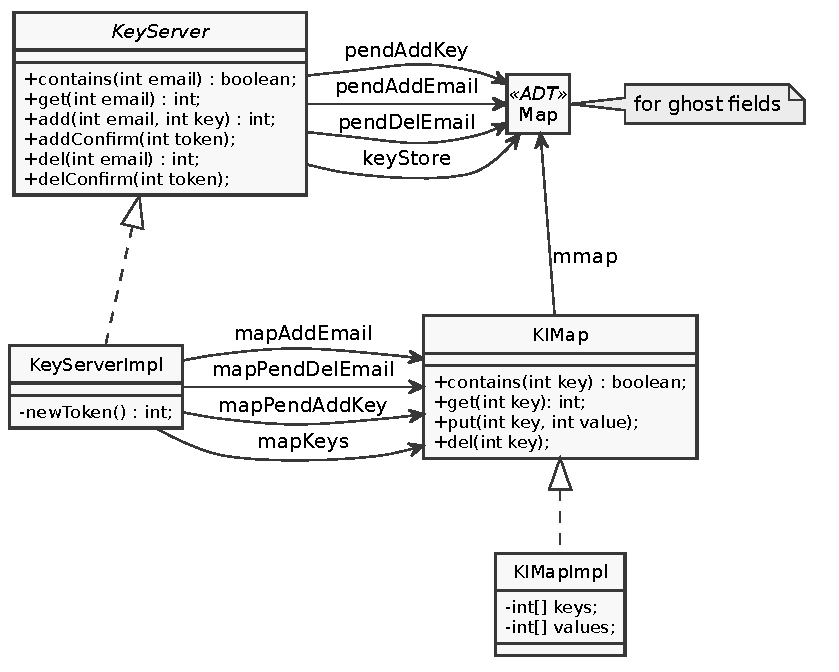
\includegraphics[height=.9\textheight]{imap}
\end{frame}

\begin{frame}[fragile]
  \frametitle{The map model}
\begin{lstlisting}
/*@ public normal_behaviour
  @  requires true;
  @  ensures keyStore == \old(keyStore);
  @  ensures pendAddEmail == \dl_mapUpdate(\old(pendAddEmail), \result, id);
  @  ensures pendAddKey == \dl_mapUpdate(\old(pendAddKey), \result, pkey);
  @  ensures pendDelEmail == \old(pendDelEmail);
  @  ensures !\dl_inDomain(\old(pendAddEmail), \result);
  @  assignable footprint;
  @*/
public int add(int id, int pkey);
\end{lstlisting}
\end{frame}

\begin{frame}[fragile]
  \frametitle{The map model}
\begin{lstlisting}[mathescape=true]
/*@ public normal_behaviour
  @  requires true;
  @  ensures keyStore == \old(keyStore);
  @  ensures pendAddEmail == \old(pendAddEmail)[\result := id];
  @  ensures pendAddKey == \old(pendAddKey)[\result := pkey];
  @  ensures pendDelEmail == \old(pendDelEmail);
  @  ensures !\result \in \old(pendAddEmail);
  @  assignable footprint;
  @*/
public int add(int id, int pkey);
\end{lstlisting}
\end{frame}



\end{document}
